\documentclass[../main.tex]{subfile}
\begin{document}
\section{Using the force field}
    If you now intend to use this force field information you can simply sample the force at a location. Then use the timestep to 
    move the actor according to the force it should have at this location for the next frame. This is done for exemple
    in the wind tail actor \texttt{BP\_WindTail}.

    \subsection{Optimising the use}
    So we have seen how the use of \texttt{BP\_WindManager::GetWindAtLocation} methode scales linearly with the number of extrema and boost.
    For this reason we are not going for every tail to sample the force field on each tick.
    Instead we can compute it every second and store it in a variable
    that we can use.

    \begin{figure}[H]
        \centering
        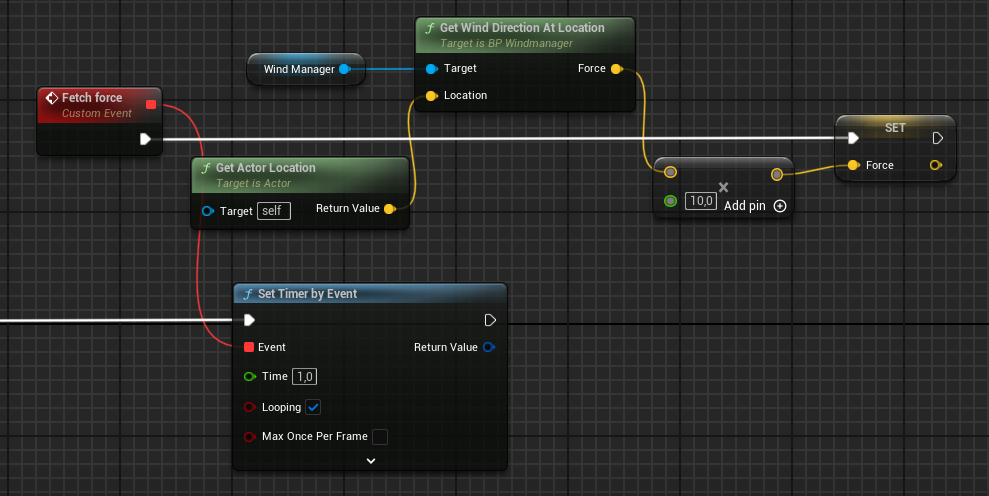
\includegraphics[width=.7\textwidth]{Ressources/TailUpdateForce.png}
        \caption{The timer updates the force at the time $t_s$, we compute the force at the location $\bm{r}(t_s)$. A factor of $10$ is used. You can modify it as you want to.}
    \end{figure}
    
    \subsection{Implementation of the motion}
    Using Eq.\ref{eq:position} we can derive the following descritied formula, which means it works for finite time steps and not infinitesimal 
    small ones like in the real life. The time step can be seen as the time between two frames $\Delta_t$ if we wish to update at each frame.
    \begin{equation}
        \bm{r}(t+\Delta_t) = \frac{1}{2} \Delta_t^2 \cdot \bm{F}_{\text{wind}}(\bm{r}(t_s)) + \Delta_t \cdot \bm{v}(t)+  \bm{r}(t)
    \end{equation}
    We can make a few observations. First the velocity is the position difference between the two updates divided by the time passed.
    we then have $\bm{v}(t) = \left(\bm{r}(t) - \bm{r}(t-\Delta_t)\right) / \Delta_t$.\\

    Second in the formal dervation we saw that the acceleration has to be multiplied with the square of the time the system lives $t^2$. This is because we add the
    acceleration to the \textit{spawn} position of the system $\bm{r}_0$. Here however we add to the position \textit{of the previous frame}. This means if we multiply by the simulation 
    time $t$ to the square, the acceleration is going to play a way to inportant role which will be incorect. For this reason we use the time step $\Delta_t$. \\
    Putt in a different way, the total displacement information in the first case is stored in the total time regarding the spawn position. In the second case
    this information is stored in the previous position so we just need a tiny shift by the acceleration. The same observation is or the velocity $\bm{v}_0$.\\

    In Eq.\ref{eq:position} the accceleration is describing the whole motion of the system involving an initial velocity but here the motion is mainly stored in the position.
    We only use the velocity to shift a bit the position and it's going to be implicitly stored in the position on the next frame.\\
    \begin{figure}[H]
        \centering
        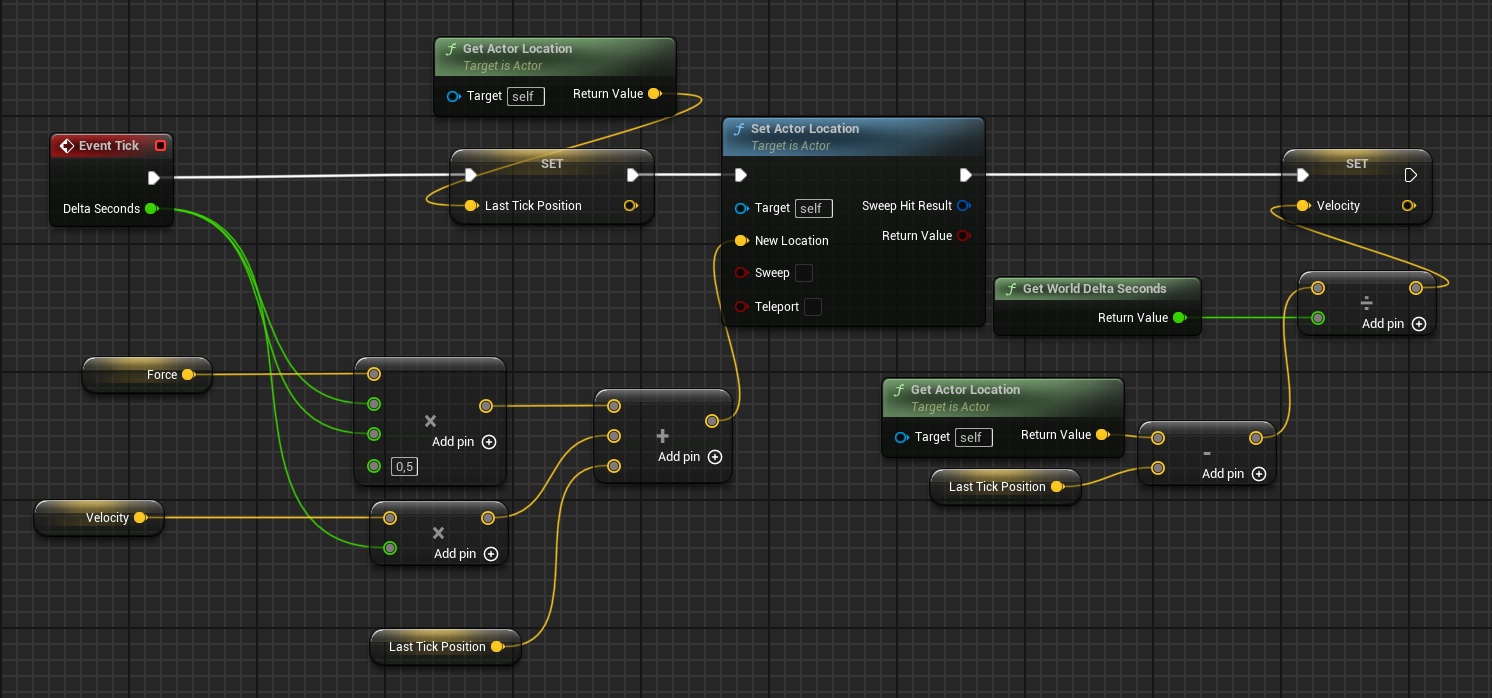
\includegraphics[width=1\textwidth]{Ressources/TailUpdateLocation.png}
        \caption{A the frame $t+\Delta_t$ we multiply the acceleration by $0.5\Delta_t^2$, the velocity with $\Delta_t$ and add it to the location from the previous update $\bm{r}(t)$. 
        \textit{After} the translation we update the velocity to be used on the next frame. If we update the velocity before the translation we are going to have $\bm{r}(t) - \bm{r}(t) = 0$.
        The last tick postion variable is used to compare before and after the update.}
    \end{figure}

    \subsection{Moving the tail around its center}
    To achieve a more complexe motion we can decide to move the particle system around the tail center. This can be changed in \texttt{BP\_WindTail} as the variable \texttt{Type}.
     For exemple the \texttt{SwingZ} mode makes the system having a vertical
    oscillation during the travel. One could also rotate the system around the propagation axis to make a spiral or simply let the line follow the current by doing nothing.\\

    \paragraph{SwingZ mode}
    This methode uses a sinusoidal function to make the tail oscillate along the $z$-axis of the tail. 
    \[
        \bm{r}_{\text{niag}}(t) = I_z\cdot \cos(\omega t + \varphi) \cdot \begin{pmatrix}0\\0\\1\end{pmatrix} + \bm{r}_{\text{tail}}(t) 
    \]
    The niagara system attached to the actor moves relatively to the actor iteself.
    $\bm{r}_{\text{tail}}(t)$ is calculated in the tick by the derivation we just made.
    \begin{figure}[H]
        \centering
        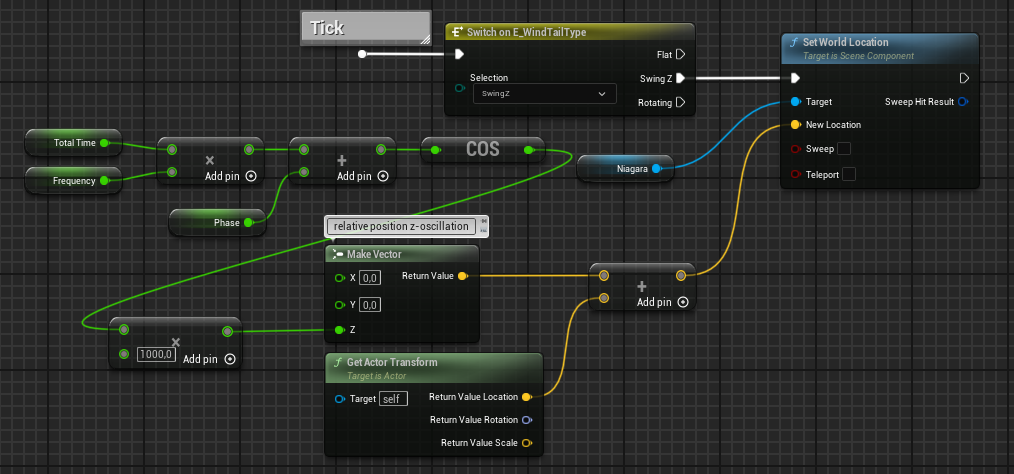
\includegraphics[width=1\textwidth]{Ressources/TailSwingZ.png}
        \caption{The tail is moving around the center of the actor. The oscillation is done by a sinusoidal function.}
    \end{figure}
    \paragraph{Spiral rotation mode}
    Here we use the up and right vector of the facing direction of the force. The oscillation will then modulate the strength of each axis. Puting the same phase $\varphi$ results
    in a cricular rotation. Varying this parameter will interpolate the rotation between a diagonal to a ellipse and then a cricle. More exemple can be found at \url{https://www.idex-hs.com/resources/resources-detail/understanding-polarization} 
    at section $a.$
    \[
        \bm{r}_{\text{niag}}(t) = I\cdot \cos(\omega t + \varphi) \cdot \hat{\bm{e}}_{\text{up}} + I\cdot \sin(\omega t + \varphi) \cdot \hat{\bm{e}}_{\text{right}}+ \bm{r}_{\text{tail}}(t) 
    \]
    with $I$ the amplitude of the oscillation and $\hat{\bm{e}}_{\text{up}}$ and $\hat{\bm{e}}_{\text{right}}$ the up and right vector of the facing direction of the force.
    \begin{figure}[H]
        \centering
        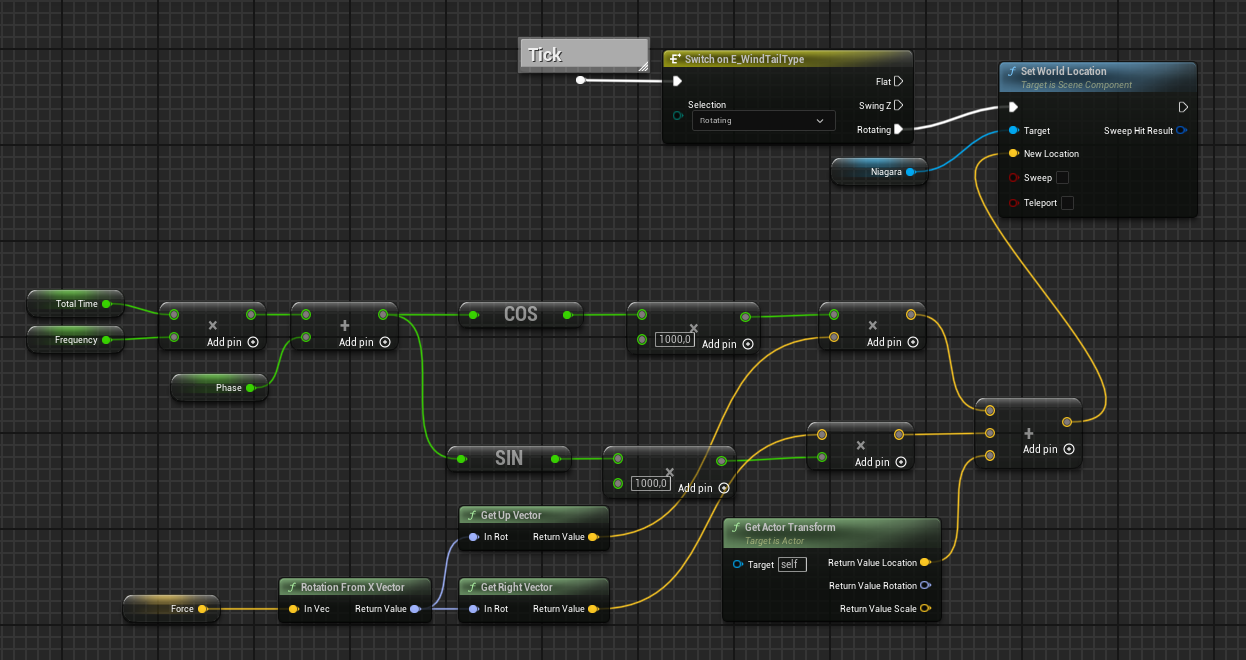
\includegraphics[width=1\textwidth]{Ressources/TailRotation.png}
        \caption{The particle is moving around the center of the tail. The rotation is done by a different sinusoidal function on each axis, perpendicular to the movement direction of
        the tail.}
    \end{figure}
    The function \texttt{BP\_WindTail::PrintRoationArrows} can be used to visualise the rotation components of the tail.  

    \subsection{The tail lifetime cycle}
    The tail spawns arround the player and move for a random time. After reaching the end of its life, the particle stops progressively and the actor is 
    teleported back in the neighborhood of the player. The parameter are redefined in a random way to achieve more diversity. The event \texttt{BP\_WindTail::RetraceAtSpawn}
    is used for this purpose. The event calls back itself after the lifecycle of the tail is over. 
\end{document}